\documentclass[11pt,a4paper]{article}
\usepackage[T1]{fontenc}
\usepackage[utf8]{inputenc}
\usepackage{lmodern}
\usepackage[a4paper,margin=22mm,headheight=16pt,footskip=12mm]{geometry}
\usepackage{microtype,amsmath,amssymb,amsthm,mathtools,bm}
\usepackage{booktabs,longtable,tabularx,array,multirow}
\usepackage{xcolor,graphicx,fancyhdr,titlesec,enumitem}
\usepackage{tikz}
\usetikzlibrary{arrows.meta,positioning}
\usepackage{listings,needspace}
\usepackage{hyperref}
\hypersetup{colorlinks=true,linkcolor=black,citecolor=black,urlcolor=black,
 pdftitle={WANTWOMAN},pdfauthor={Tom Klootwijk; AI-assisted formalization},
 pdfsubject={Unified approximation of multiscale cyclic dynamics, recursive geometry, and one-bit physical-field encoding},
 pdfkeywords={WANTWOMAN, Pinion Double Hadamard, OTAN2, PSI Fork Razor, P64, fixed point}}
\definecolor{ink}{HTML}{152B39}
\definecolor{muted}{HTML}{52636E}
\definecolor{rulegray}{HTML}{B8C2C8}
\definecolor{papergray}{HTML}{F3F5F6}
\setlength{\parindent}{0pt}
\setlength{\parskip}{6pt plus 1pt}
\setlength{\emergencystretch}{2em}
\setcounter{tocdepth}{1}
\renewcommand{\arraystretch}{1.15}
\pagestyle{fancy}
\fancyhf{}
\fancyhead[L]{\sffamily\small\bfseries WANTWOMAN}
\fancyhead[R]{\sffamily\small Formalization / 1.0}
\fancyfoot[L]{\sffamily\footnotesize Tom Klootwijk}
\fancyfoot[R]{\sffamily\footnotesize\thepage}
\renewcommand{\headrulewidth}{0.3pt}
\titleformat{\section}{\Large\sffamily\bfseries\color{ink}}{\thesection}{0.65em}{}
\titleformat{\subsection}{\large\sffamily\bfseries\color{ink}}{\thesubsection}{0.6em}{}
\titleformat{\subsubsection}{\normalsize\sffamily\bfseries}{\thesubsubsection}{0.6em}{}
\titlespacing*{\section}{0pt}{18pt}{9pt}
\titlespacing*{\subsection}{0pt}{12pt}{5pt}
\newtheorem{proposition}{Proposition}[section]
\newtheorem{definition}[proposition]{Definition}
\newtheorem{theorem}[proposition]{Theorem}
\newcommand{\R}{\mathbb{R}}
\newcommand{\Z}{\mathbb{Z}}
\newcommand{\B}{\{0,1\}}
\newcommand{\ind}{\mathbf{1}}
\newcommand{\diag}{\operatorname{diag}}
\newcommand{\clip}{\operatorname{clip}}
\newcommand{\round}{\operatorname{rnd}}
\newcommand{\fracpart}{\operatorname{frac}}
\newcommand{\wrap}{\operatorname{wrap}}
\newcommand{\sgn}{\operatorname{sgn}}
\newcommand{\OT}{\operatorname{OTAN2}}
\newcommand{\Source}{\textsf{S}}
\newcommand{\Def}{\textsf{D}}
\newcommand{\Phys}{\textsf{E}}
\newcommand{\tagline}[1]{\par\smallskip{\small\sffamily\color{muted}#1}\par\smallskip}
\newcommand{\sourcepage}[1]{\cite[pp.~#1]{source}}
\newcommand{\onepage}{\clearpage}
\numberwithin{equation}{section}
\lstset{basicstyle=\ttfamily\small,columns=fullflexible,keepspaces=true,
 breaklines=true,frame=single,rulecolor=\color{rulegray},backgroundcolor=\color{papergray},
 showstringspaces=false,tabsize=4,aboveskip=9pt,belowskip=9pt}
\newcolumntype{Y}{>{\raggedright\arraybackslash}X}

\begin{document}
\begin{titlepage}
\thispagestyle{empty}
{\sffamily\small\bfseries TECHNICAL FORMALIZATION\hfill EDITION 1.0}
\vspace{18mm}
{\color{ink}\rule{\textwidth}{1.4pt}}
\vspace{7mm}
{\sffamily\bfseries\fontsize{40}{45}\selectfont WANTWOMAN\par}
\vspace{9mm}
{\sffamily\Large Tom Klootwijk's unified approximation of\par}
\vspace{4mm}
{\sffamily\LARGE\bfseries Multiscale cyclic dynamics,\\[2mm]
recursive geometry, and\\[2mm]
one-bit physical-field encoding\par}
\vspace{12mm}
{\large\bfseries Tom Klootwijk\par}
{\large NL200678942\par}
{\large 10-07-1990\par}
\vspace{4mm}
{\small Identification and birth date reproduced as supplied by the author.}
\vfill
\begin{tabularx}{\textwidth}{@{}p{37mm}Y@{}}
\toprule
Formal core & Pinion Double Hadamard operator; binary bifurcation; logarithmic polar coordinates; OTAN2; Klein chart closure; PSI Fork Razor.\\
Implementation & A fully specified 64-bit node profile, one-bit output, Python reference kernel, conformance tests and reproducible synthetic data.\\
Physical supplement & Mechanics, oscillation, conservation, transport, electromagnetism, quantum evolution, relativity and crop-water coupling.\\
\bottomrule
\end{tabularx}
\vspace{8mm}
{\sffamily\small 15 September 2026\hfill Source-based, AI-assisted edition}
\end{titlepage}

\section*{Formal statement}
\addcontentsline{toc}{section}{Formal statement}
\textbf{The blank is filled as follows:}
\begin{quote}
\large A unified approximation of multiscale cyclic dynamics, recursive geometry, and one-bit physical-field encoding.
\end{quote}
WANTWOMAN is defined here as a \emph{coupled representation and transition system}: dimensioned physical or measured inputs are normalized, combined with recursive node geometry, encoded into a versioned word, transformed in a stated order, and reduced to a binary observation. The uploaded 21-page source supplies the architecture and its terminology. This edition supplies the missing domains, units, arithmetic semantics, boundary conditions and test procedures. The physical equations are identified separately from the source-derived computational rules.

\begin{equation}
\boxed{\begin{aligned}
u_{n+1}&=\mathcal F_{h,j}(u_n;\eta_n),\\
(W_{n+1},O_{n+1})&=\mathcal K_{\Theta}
\bigl(W_n,O_n;\mathcal E_j(u_{n+1}),b_n\bigr).
\end{aligned}}
\label{eq:master}
\end{equation}
Here $u_n$ is the selected physical state, $j$ selects its governing equation, $\eta_n$ supplies boundary or forcing data, $\mathcal F_{h,j}$ is a specified physical time step, $\mathcal E_j$ is its normalization/encoding adapter, $b_n\in\B$ selects a tree branch, and $\Theta$ is the complete configuration. The node word is $W_n\in\{0,\ldots,2^{64}-1\}$ and the occupancy output is $O_n\in\B$.

The equality in \eqref{eq:master} is a definition of the coupled architecture. A physical evolution rule, an encoding rule, and a geometric transformation remain individually identifiable. This makes numerical behavior reproducible and conservation laws testable.

\subsection*{Reading conventions}
\begin{tabularx}{\textwidth}{@{}p{16mm}Y@{}}
\toprule
\textsf{S} & A convention or term retained from the supplied source.\\
\textsf{D} & A definition, completion, parameter choice or explicit correction introduced in this edition.\\
\textsf{P} & A mathematical proposition proved from its stated assumptions.\\
\textsf{E} & An established physical equation imported from the cited external source.\\
\textsf{T} & A check actually executed by the accompanying implementation.\\
\bottomrule
\end{tabularx}
The source's original pages are preserved in the archive. Section~\ref{sec:ledger} records the important differences between its prose, displayed mathematics and code. No biological periods, measured material constants, fitted experimental results or genealogical information are inferred from the name, identifier or birth date.

\onepage
\tableofcontents
\onepage

\section{Attribution, state and dimensional contract}
\label{sec:contract}
\tagline{Basis: source pp.~1--5 and 18--20. Classification: S + D.}

The framework is attributed to \textbf{Tom Klootwijk}, with identifier \textbf{NL200678942} and Gregorian birth date \textbf{1990-07-10}, as supplied in the request. The submitted file is an exported dialogue containing descriptions, equations and pseudocode; its publication filename and page references identify the source artifact \cite{source}. The mathematical completions, proofs, implementation choices and physical adapters in this edition are explicitly marked as such.

\subsection{What the complete state contains}
A node word and an output bit are not the complete memory of a scene. Define
\begin{equation}
\begin{aligned}
S_n&=(W_n,O_n,\mathcal C_n),\\
\mathcal C_n&=(\text{clocks, LUTs, bounds, frontier, physical state, configuration}).
\end{aligned}
\end{equation}
The 64-bit promise applies to $W_n$, not to $\mathcal C_n$. A traversal address, a collection of nodes, an entire continuous field and several independent clocks cannot be recovered from an unspecified single word. The profile identifier is external metadata and must accompany serialized words.

\subsection{Normalization before algebra}
Let physical position be $\bm x$ in metres, time $t$ in seconds and a scalar physical observable $u$ in its own unit. Select $L_*>0$, $T_*>0$ and $U_*>0$, and write
\begin{equation}
\bm q=\frac{\bm x-\bm P}{L_*},\qquad
\tau=\frac{t-t_*}{T_*},\qquad \widetilde u=\frac{u-u_*}{U_*}.
\label{eq:nondim}
\end{equation}
Only dimensionless quantities are added inside a feature transform. The fourth coordinate of the source's Hadamard vector is denoted $\zeta$ here, rather than reusing $\phi$ for both a coordinate and the golden ratio. A four-component feature vector is not, merely by having four entries, a relativistic spacetime vector.

\begin{tabularx}{\textwidth}{@{}p{23mm}p{33mm}Y@{}}
\toprule
Symbol & Domain / unit & Meaning\\
\midrule
$\phi,\alpha$ & dimensionless; radians & Golden ratio and golden angular increment.\\
$\ell,r,\vartheta$ & real; integer codes & Log radius, stored radial code, stored angular code.\\
$\rho_m,\rho_e$ & $\mathrm{kg\,m^{-3}}$; $\mathrm{C\,m^{-3}}$ & Physical mass and charge density; not the radial code.\\
$\chi,\kappa,O$ & bits & Symbolic label/parity control, chart orientation, output.\\
$d,p,j_L$ & integer indices & Tree depth, 5-bit phase bin and 7-bit LUT address.\\
$\Gamma_\epsilon$ & dimensionless & Regularized logarithmic modulation, not a gravitational connection.\\
\bottomrule
\end{tabularx}

\subsection{Runtime arithmetic policy}
The P64 node kernel uses integers, additions, subtractions, comparisons, bit operations and division by powers of two with a fixed rounding rule. Its fixed golden-ratio products are implemented by shift-and-add. It performs no runtime coordinate squaring or trigonometric evaluation. Physical equations retain their conventional products and powers; compiling an operation changes its numerical implementation, not the equation's meaning. Exact symbolic algebra, finite arithmetic and empirical calibration are separate stages.

\section{The constants, Gregorian anchor and clocks}
\label{sec:constants}
\tagline{Basis: source p.~1 and phase descriptions on pp.~2--5. Exact numerical links are supplied in this edition.}

\subsection{A precise connection among 3.6, 36, phi and a full turn}
Set
\begin{equation}
\phi=\frac{1+\sqrt5}{2},\qquad \phi^{-1}=\phi-1,\qquad
\alpha=\frac{2\pi}{\phi^2}=2\pi(2-\phi).
\label{eq:phi}
\end{equation}
A deliberately chosen 100-step angular lattice gives
\begin{equation}
\Delta\theta=3.6^\circ=\frac{\pi}{50},\qquad
10\Delta\theta=36^\circ=\frac{\pi}{5},\qquad
100\Delta\theta=360^\circ=2\pi.
\end{equation}
The exact fivefold-symmetry identity is
\begin{equation}
2\cos(36^\circ)=\phi,\qquad 2\cos(72^\circ)=\phi^{-1}.
\end{equation}
For example, let $x=2\cos(\pi/5)$. The triple- and double-angle identities give
$x^3-3x=-(x^2-2)$, so $(x+2)(x^2-x-1)=0$. Since $x>0$, $x=\phi$. This links the named angular quantities exactly; a choice of angular unit remains part of the statement.

There is also an independent exact physical-unit conversion:
\begin{equation}
\frac{v}{\mathrm{km\,h^{-1}}}=3.6\,\frac{v}{\mathrm{m\,s^{-1}}},
\qquad 3.6=\frac{3600}{1000}.
\end{equation}
The number $36$ used as a completed age, $36^\circ$ used as an angle and a count of 36 updates are different typed quantities. Their numerical equality does not remove their different units or roles.

\subsection{Fibonacci recursion and its exact approximation}
\begin{equation}
F_0=0,\quad F_1=1,\quad F_{n+2}=F_{n+1}+F_n,\qquad
\begin{pmatrix}F_{n+1}\\F_n\end{pmatrix}
=\begin{pmatrix}1&1\\1&0\end{pmatrix}^{n}\begin{pmatrix}1\\0\end{pmatrix}.
\end{equation}
The recursion matrix has eigenvalues $\phi$ and $-\phi^{-1}$; diagonalization yields
\begin{equation}
F_n=\frac{\phi^n-(-\phi^{-1})^n}{\sqrt5},\qquad
\lim_{n\to\infty}\frac{F_{n+1}}{F_n}=\phi.
\end{equation}
Thus a rational approximant may be chosen as $F_{n+1}/F_n$. A single left shift multiplies an integer by two, not by $\phi$. The source's alternating shifts are retained as optional scale operations, not as an identity for golden-ratio multiplication.

\subsection{The civil-date anchor}
For any valid Gregorian date $(Y,M,D)$ on or after the supplied birth date,
\begin{equation}
A(Y,M,D)=Y-1990-\ind\{(M,D)<(7,10)\}.
\end{equation}
Consequently $A(2026,7,10)=A(2026,9,15)=36$. The civil-date difference from 10 July 1990 to 10 July 2026 is 13,149 days. The birth time and time zone are not supplied, so this date anchor sets neither an exact elapsed SI-second count nor a physical phase origin.

\subsection{Phase is not the Fourier transform}
A normalized cyclic phase and a Fourier transform are defined separately:
\begin{align}
\psi_j(t)&=\fracpart\!\left(\psi_{j,0}+\int_{t_*}^{t}f_j(s)\,ds\right)\in[0,1),\\
\widehat g(\nu)&=\int_{-\infty}^{\infty}g(t)e^{-2\pi i\nu t}\,dt.
\end{align}
The source name \texttt{FT\_sweep} is retained as the phase field's historical label; its stored content is $p=\lfloor32\psi\rfloor$. If $f_j$ has units $\mathrm{s^{-1}}$, its integral is dimensionless. A transform of a signal requires that signal and an integrability or distributional convention; a linear ramp alone does not define one.

\subsection{Biological/agricultural modulation as supplied input channels}
The source uses gestation, crop and menstruation channels \sourcepage{2--4}. Complete its logarithmic expression with
\begin{equation}
\Gamma_\epsilon(t)=\log\!\left(\max\left\{\epsilon,
\left|\sin(2\pi\psi_g)\cos(2\pi\psi_c)\sin(2\pi\psi_m)\right|\right\}\right)+\xi(t),
\quad 0<\epsilon\le1.
\label{eq:modulation}
\end{equation}
For $|\xi|\le J$, $\log\epsilon-J\le\Gamma_\epsilon\le J$. This regularization removes the source expression's $\log0$ singularity. It does not make $\Gamma_\epsilon$ nonnegative. Define an integer forcing adapter by
\begin{equation}
\gamma_n=\clip_{[-31,31]}\!\left(\round(g_*\Gamma_\epsilon(t_n))\right),
\end{equation}
with declared gain $g_*$. Measured phases, event timestamps, channel periods and jitter seeds belong in the configuration. A one-off duration may instead use progress
$\psi_g=\clip_{[0,1]}((t-t_{g,0})/T_g)$ without periodic reset. This avoids silently turning a finite event into a repeating oscillator.

An exact rational clock with $P$ ticks per cycle stores an external counter $a$:
\begin{equation}
a_{n+1}=(a_n+1)\bmod P,\qquad p_n=\left\lfloor\frac{32a_n}{P}\right\rfloor.
\end{equation}
Its period is exactly $Ph$. Only its current five-bit phase is copied into the node word.

\section{Pinion nuclei, log-polar coordinates and binary fields}
\label{sec:geometry}
\tagline{Basis: source pp.~2--5 and 13--17. Classification: S + D.}

\subsection{Coordinates about a moving nucleus}
For a local planar position $\bm x\ne\bm P_i(t)$, select a positive reference length $R_*$ and define
\begin{equation}
r_{\rm phys}=\|\bm x-\bm P_i(t)\|_2,\quad
\ell=\log_2(r_{\rm phys}/R_*),\quad
\theta=\arg(\bm x-\bm P_i(t))\pmod{2\pi}.
\end{equation}
The inverse chart is
\begin{equation}
\bm x=\bm P_i(t)+R_*2^\ell(\cos\theta,\sin\theta),
\qquad r_{\rm phys}>0.
\end{equation}
Changing to log-polar coordinates changes the representation, not the intrinsic curvature of an otherwise Euclidean plane. The origin is a separate nucleus case: $r_{\rm phys}=0$ has no finite log radius. A compiler must branch on that case or record it outside the radial word; replacing it by a small positive radius is an explicit approximation.

The default radial quantizer is
\begin{equation}
r=\clip_{[0,2047]}\!\left(\round\frac{\ell-\ell_{\min}}{\Delta\ell}\right),\quad
\ell_{\min}=-8,\quad\Delta\ell=\frac1{128},\quad
\widehat\ell=-8+\frac{r}{128}.
\label{eq:radial}
\end{equation}
Thus $r=1024$ means $r_{\rm phys}=R_*$, not zero radius. The auxiliary axial code $z$ may be decoded as $x_z=L_z z$ when an axial scale $L_z$ is specified. Integer feature mixing is performed after these physical interpretations have been normalized.

\subsection{The field's sign and the field's distance are different}
For a real implicit function $f_i$, define
\begin{equation}
O_i(\bm q)=\ind\{f_i(\bm q)\le0\},\qquad
O_{\cup}=\bigvee_i O_i,\quad O_{\cap}=\bigwedge_i O_i,\quad
O_{\triangle}=\bigoplus_i O_i.
\end{equation}
These represent union, intersection and parity/symmetric difference. The source uses both OR and XOR; they are separate scene-composition policies. An occupancy bit contains a sign decision, not a signed distance magnitude.

For a set $\Omega$ with chosen metric $d$, an actual signed distance is
\begin{equation}
\operatorname{sd}_{\Omega}(\bm q)=
\begin{cases}-d(\bm q,\partial\Omega),&\bm q\in\Omega,\\
+d(\bm q,\partial\Omega),&\bm q\notin\Omega.
\end{cases}
\end{equation}
The source name ``1-bit SDF'' is used here only as a historical label for the sign/occupancy stage. Distances used for geometric bounds must be supplied separately.

\subsection{Primitive predicates without coordinate squaring}
Several useful shapes have direct predicates:
\begin{align}
O_{\rm apex}&=\ind\{|x|+|y|+|z|\le\epsilon_a\},\\
O_{\rm pyramid}&=\ind\{0\le z\le H,\ |x|+|y|\le a z\},\\
O_{\rm box}&=\ind\{\max(|x|/a,|y|/b,|z|/c)\le1\}.
\end{align}
Here all coordinates and parameters are normalized. The first set is an $L^1$ ball around the apex; the second is a finite diamond-cross-section pyramid with apex at $z=0$. The source's $|x|+|y|-|z|\le0$ instead describes an unbounded double pyramid.

A Euclidean ball can be defined by support inequalities,
\begin{equation}
\|\bm q\|_2\le R\quad\Longleftrightarrow\quad
\bm n\cdot\bm q\le R\ \ \text{for every unit vector }\bm n.
\end{equation}
A finite set of normals gives a polyhedral approximation. A one-angle planar LUT describes a radial boundary in two dimensions; a general three-dimensional sphere/surface requires its dimensional interpretation or additional angular/axial data. Neither $\log|x|+\log|y|$ nor an arbitrary one-angle lookup alone proves spherical geometry.

\subsection{Golden leaves and optional radial laws}
Retain the source's leaf-angle convention
$\theta_n=2\pi n/\phi\pmod{2\pi}$. Since $1/\phi+1/\phi^2=1$, this is the opposite orientation of $n\alpha$. Either orientation may be selected explicitly. Two completed radial choices are
\begin{equation}
\text{log spiral: }\ell_n=\ell_0-n\log_2\phi;
\qquad
\text{equal-area planar sampling: }r_n=a\sqrt{n+\eta},\quad\eta>0.
\end{equation}
These are different generators, not two names for the same curve. The source does not choose a complete radial law. The integer kernel's golden increments are modulated by other features; its full trajectory is therefore not identified with the unmodulated leaf sequence.

\section{The Pinion Double Hadamard operator}
\label{sec:pinion}
\tagline{Basis: displayed operator on source p.~5; integer cross-additions on p.~9. Classification: S + D + P.}

\subsection{Exact real operator}
Set
\begin{equation}
H_2=\frac1{\sqrt2}\begin{pmatrix}1&1\\1&-1\end{pmatrix},\qquad
H_4=H_2\otimes H_2=\frac12 M,
\end{equation}
\begin{equation}
M=\begin{pmatrix}
1&1&1&1\\1&-1&1&-1\\1&1&-1&-1\\1&-1&-1&1
\end{pmatrix},\qquad
D_\phi=\diag(\phi,\phi^{-1},1,-1),\qquad A=D_\phi H_4.
\label{eq:pinion}
\end{equation}
The source's componentwise notation $(H_4\bm v)\odot\bm p$ is exactly $A\bm v$ when $\bm p=(\phi,\phi^{-1},1,-1)^T$. Matrix multiplication, Kronecker product and componentwise product are distinct operations.

\begin{proposition}[Hadamard and pinion invariants]
$H_4^T H_4=I$, $H_4^2=I$, $\det H_4=1$, $\det A=-1$ and $|\det A|=1$. The singular values of $A$ are $\phi,1,1,\phi^{-1}$. Thus $A$ preserves four-dimensional volume magnitude, while generally changing lengths and areas.
\end{proposition}
\begin{proof}
Every row of $M$ has squared length four and different rows have zero dot product, so $M^TM=4I$. Symmetry gives $H_4^2=I$. The Kronecker determinant identity gives $\det(H_2\otimes H_2)=(-1)^2(-1)^2=1$. Also $\det D_\phi=-1$. Finally $AA^T=D_\phi^2$, whose positive square-root eigenvalues give the stated singular values.
\end{proof}
A useful explicit counterexample to length preservation is $\bm v=H_4\bm e_1$. It has unit length, whereas $A\bm v=\phi\bm e_1$ has length $\phi$. The full pinion operator is therefore not orthogonal. Nor is it positive definite or, in general, an involution. Its four-dimensional determinant does not by itself prove three-dimensional physical-volume preservation.

\subsection{A bounded branching version}
For finite geometry, define $T_b(\bm v)=sA\bm v+\bm t_b$ with $s>0$. Since the largest absolute row sum of $A$ is $2\phi$,
\begin{equation}
\|T_b(\bm v)-T_b(\bm w)\|_\infty\le 2s\phi\|\bm v-\bm w\|_\infty.
\end{equation}
Selecting $s=1/4$ yields contraction factor $a=\phi/2<1$. If $\|\bm t_b\|_\infty\le\beta$, induction gives
\begin{equation}
\|\bm v_n\|_\infty\le a^n\|\bm v_0\|_\infty+
\beta\frac{1-a^n}{1-a}.
\end{equation}
This is a bounded affine branch model. The wrapped/clipped integer kernel in Section~\ref{sec:kernel} is separately defined; it is not assigned this real-map contraction theorem after discontinuous wrapping.

\subsection{A precise finite implementation}
Use nearest-integer rounding with ties away from zero:
\begin{equation}
\round(x)=\sgn(x)\lfloor |x|+1/2\rfloor,\qquad\round(0)=0.
\end{equation}
The default binary approximants are
\begin{equation}
\phi_Q=\frac{106039}{65536}=1.6180267333984375,
\quad \iota_Q=\frac{40503}{65536}=0.6180267333984375.
\end{equation}
Each differs from its exact target by approximately $7.25535\times10^{-6}$. Their product is $0.999983776593580842\ldots$, not exactly one. Accordingly the compiled pinion is not assigned exact volume preservation.

The ordered integer transform is
\begin{align}
h_i&=\round\bigl((M\bm v)_i/2\bigr),\\
\bm a&=\bigl(\round(106039h_0/65536),\ \round(40503h_1/65536),\ h_2,\ -h_3\bigr),\\
u_i&=\round(a_i/4).
\label{eq:integerpinion}
\end{align}
Each stage uses widened integers before field limits are applied. Multiplication by an integer $c=\sum_kc_k2^k$ is exactly $cx=\sum_{k:c_k=1}(x\ll k)$ with sign handled separately. An odd cross-sum creates a half-integer before rounding; losing that half-bit prevents an exact inverse in general.

The golden increments used by P64 are
\begin{equation}
g_{11}=\round(2048/\phi^2)=782,\qquad
 g_{10}=\round(1024/\phi^2)=391.
\end{equation}
The 11-bit angular increment differs from $\alpha$ by approximately $8.17277\times10^{-4}$ radians per unwrapped addition. Reducing modulo a turn does not eliminate accumulated phase error.

\section{Binary bifurcation and the PSI Fork Razor}
\label{sec:psi}
\tagline{Basis: source pp.~2--3, 5--7 and 10. Classification: S + D + P.}

\subsection{Tree semantics}
The abstract nodes are finite binary strings $w\in\B^*$, with root $\varepsilon$ and children $w0,w1$. The depth is $|w|$. This is a rooted binary tree. It becomes a \emph{binary search tree} only when an ordered key and search invariant are also specified; the uploaded source supplies neither. WANTWOMAN retains ``BST'' as a historical field name for the depth.

A tree boundary can carry a genuine ultrametric: for infinite paths $a,b$ and longest common prefix length $\ell(a,b)$, set
\begin{equation}
d_T(a,b)=2^{-\ell(a,b)}\quad(a\ne b),\qquad d_T(a,a)=0.
\end{equation}
Because two paths sharing prefixes with a third share at least the shorter prefix with one another, $d_T(a,c)\le\max\{d_T(a,b),d_T(b,c)\}$. This supplies a precise interpretation of the source's non-Archimedean language on \emph{tree addresses}, rather than deriving such a metric from $|x|+|y|$.

The runtime depth is $0\le d\le31$. A full tree through depth 31 has $2^{32}-1$ nodes; a depth-first traversal needs a separate frontier or address. Indefinitely many time steps can be generated by reusing records, while finite memory still has finitely many states.

\subsection{The exact culling invariant}
Let $G_w$ be all geometry owned by node $w$, and require an enclosure
\begin{equation}
C_w\supseteq\bigcup_{v\succeq w}G_v.
\label{eq:subtreecontainment}
\end{equation}
The observing slit is
\begin{equation}
P_{\bm n,c,\delta}=\{\bm x:|\bm n\cdot\bm x-c|\le\delta\},\qquad
\delta\ge0.
\end{equation}
For $C_w=\prod_i[l_i,u_i]$, set
\begin{equation}
L=\sum_i\min(n_i l_i,n_i u_i)-c,\qquad
U=\sum_i\max(n_i l_i,n_i u_i)-c.
\end{equation}
\begin{theorem}[PSI Fork Razor]
Under \eqref{eq:subtreecontainment}, the test $L>\delta$ or $U<-\delta$ permits the entire subtree to be discarded without losing any geometry intersecting the slit.
\end{theorem}
\begin{proof}
Every descendant point is in $C_w$, and every point in $C_w$ has signed slit coordinate in $[L,U]$. Under the stated test this interval misses $[-\delta,\delta]$, so every descendant misses the slit.
\end{proof}
This is a slice-intersection proof, not an occlusion or hidden-surface proof. An enclosure of the parent primitive alone is insufficient: a parent at $x=2$ with a child translated by $-2$ misses $x=0$, but the child reaches it. The source test $|x|>32-d$ requires a proved remaining-displacement bound in the same coordinate units; depth alone supplies no such bound.

\subsection{Constructing the enclosures}
For an affine transform $T(\bm x)=B\bm x+\bm t$, the exact interval image bounds are
\begin{equation}
\underline y_i=t_i+\sum_j\min(B_{ij}l_j,B_{ij}u_j),\qquad
\overline y_i=t_i+\sum_j\max(B_{ij}l_j,B_{ij}u_j).
\end{equation}
A bottom-up finite tree can store
\begin{equation}
C_w=\operatorname{hull}\bigl(G_w,T_0(C_{w0}),T_1(C_{w1})\bigr)
\end{equation}
when the children are expressed in their corresponding local charts. The package supplies exact rational interval operations and tests them on an enumerated depth-six branch system. For floating-point bounds, outward rounding is required; for wrapped angular intervals, split at the seam or use the whole angular range. Applying an unwrapped interval proof to wrapped codes would violate its assumptions.

The node kernel has no implicit culling shortcut. A scene compiler must supply validated descendant bounds before invoking the PSI stage. When those bounds are absent, the reference demo retains the node.

\section{Klein closure, parity and local occupancy}
\label{sec:klein}
\tagline{Basis: source pp.~6, 8--9, 11--14 and 17. Classification: S + D + P; quotient construction referenced to Hatcher.}

\subsection{A Klein bottle requires an identification rule}
Define the Klein surface as
\begin{equation}
K=([0,1]\times S^1)/\bigl((0,\theta)\sim(1,-\theta)\bigr),
\qquad\theta\sim\theta+2\pi.
\label{eq:klein}
\end{equation}
This is the rectangle construction with one pair of edges glued with reversed orientation \cite[pp.~44--45]{hatcher}. A local transverse direction reverses when carried once around the identified longitudinal cycle, so no consistent orientation extends around that loop. A vector equation with eigenvalue $-1$ is not, on its own, the equivalence relation in \eqref{eq:klein}.

For the depth clock, $u=d/32$ labels the current discrete longitudinal position; advancing the $d=31$ state crosses the $u=1$ seam and resets to $d=0$. Use a chart bit $\kappa$ to record orientation and define the seam map
\begin{equation}
\mathcal J(\vartheta,\kappa)=(-\vartheta\bmod2048,\kappa\oplus1).
\label{eq:seam}
\end{equation}
It is an involution. The depth-reset operation is separate and is not invertible without the prior traversal history. The nonterminal kernel acts on chart records that include $\kappa$ and traversal history; it is not assigned smoothness or chart-equivariance merely by using this seam. A global physical-field adapter must additionally satisfy its own transition-compatibility conditions.

\subsection{A scalar observation compatible with the seam}
Let
\begin{equation}
\vartheta_{\mathrm{eff}}=(-1)^\kappa\vartheta\pmod{2048},\quad
j_L=\bigl(\lfloor\vartheta_{\mathrm{eff}}/16\rfloor+p\bigr)\bmod128,
\quad O=\ind\{r\le L[j_L]\}.
\label{eq:lookup}
\end{equation}
\begin{proposition}[Chart-consistent occupancy]
For unchanged $r,p,L$, the observation in \eqref{eq:lookup} is invariant under $\mathcal J$.
\end{proposition}
\begin{proof}
After the seam, $(-1)^{\kappa\oplus1}(-\vartheta)=(-1)^\kappa\vartheta$ modulo 2048. Thus $\vartheta_{\mathrm{eff}}$, $j_L$ and $O$ are unchanged.
\end{proof}
This is a local radial-membership observable that descends through the identification. It does not require a global ``inside of the Klein bottle'' or a change from matter to antimatter. A Boolean encoding also does not remove geometric handedness by itself: parity, orientation and the interpretation of a scalar output are distinct pieces of data.

\subsection{The source's radial half-turn is a different map}
The polar formula on source p.~14 can be completed as the finite involution
\begin{equation}
\mathcal R(r,\vartheta,\kappa)=
(2047-r,\vartheta+1024\bmod2048,\kappa\oplus1).
\end{equation}
In physical radial coordinates it is inversion $r_{\rm phys}\mapsto C/r_{\rm phys}$ for a constant $C$ set by the endpoints of the log interval, together with a half-turn. This map is retained as \texttt{source\_polar\_involution}; it is not substituted for the Klein quotient's seam without changing the profile. It does not automatically complement the occupancy bit.

The Cartesian sign operation $(x,y,z)\mapsto(-x,y,-z)$ on source p.~6 has determinant $+1$: it is a half-turn, not a three-dimensional orientation reversal. Its nonlinear extra change $\phi\mapsto\phi^{-1}$ also prevents treating the complete displayed operation as a fixed linear matrix on arbitrary four-vectors. These distinctions are recorded rather than conflated.

\section{The exact 64-bit word profile}
\label{sec:packing}
\tagline{Basis: source p.~8 table; later polar reinterpretation on pp.~13--20. Normative profile: WANTWOMAN-P64-v1.}

\subsection{Field allocation}
The detailed table on source p.~8 is the allocation authority; its earlier schematic on p.~7 has different boundaries. This edition keeps all 64 bits and identifies the later polar interpretation explicitly.

\begin{center}\small
\begin{tabularx}{\textwidth}{@{}p{18mm}p{16mm}p{22mm}Y@{}}
\toprule
Bits & Width & Field & P64 meaning / range\\
\midrule
63 & 1 & $\chi$ & Symbolic label and phase/parity control; 0 or 1.\\
62:52 & 11 & $r$ & Unsigned offset log-radius code; 0--2047.\\
51:41 & 11 & $\vartheta$ & Unsigned angular code; 0--2047; one turn is 2048.\\
40:30 & 11 & $z$ & Signed auxiliary axial feature; $-1024$--1023.\\
29:20 & 10 & $\Phi$ & Unsigned periodic phyllotaxis feature; 0--1023.\\
19:15 & 5 & $d$ & Tree depth; 0--31.\\
14:10 & 5 & $p$ & Discrete phase bin; 0--31.\\
9:3 & 7 & $j_L$ & Polar boundary-table address; 0--127.\\
2 & 1 & $\kappa$ & Chart-orientation bit.\\
1:0 & 2 & $\Xi$ & Channel selector: 0 gestation, 1 crop, 2 menses, 3 composite/user channel.\\
\bottomrule
\end{tabularx}\end{center}
The sum is $1+11+11+11+10+5+5+7+1+2=64$. The original Cartesian interpretation uses signed $X,Y,Z$ fields instead; converting a word from Cartesian to P64 requires decoding and re-encoding, not just renaming the two leading slots. The final source schematic omits the $Z$ slot; P64 retains it as $z$.

$O$ is a separate return value, not bit~0. Bit~0 already belongs to $\Xi$. The source's assignment \texttt{sdf\_o = W \& 1} reads the low bit of the channel selector, not a separately stored occupancy result.

\subsection{Encoding and replacement}
For field $f$ of width $b_f$ and shift $s_f$, let
\begin{equation}
 m_f=(2^{b_f}-1)\ll s_f,\qquad
\operatorname{raw}_f(W)=(W\gg s_f)\mathbin{\&}(2^{b_f}-1).
\end{equation}
For a signed field with raw code $u$,
\begin{equation}
\operatorname{signed}_{b}(u)=
\begin{cases}u,&u<2^{b-1},\\u-2^b,&u\ge2^{b-1}.
\end{cases}
\end{equation}
A checked field replacement is
\begin{equation}
\operatorname{set}_f(W,v)=
(W\mathbin{\&}(M_{64}\mathbin{\oplus}m_f))\mathbin{|}
\bigl((v\mathbin{\&}(2^{b_f}-1))\ll s_f\bigr),\quad M_{64}=2^{64}-1.
\end{equation}
The API rejects values outside the declared field range. The kernel first clips $r,z$ and wraps $\vartheta,\Phi$; only then does it call the checked replacement. Its masks are generated from the allocation instead of copied from incompatible source examples.

\subsection{Negation, complement and toggling}
Two's-complement negation of a $b$-bit code is
\begin{equation}
\operatorname{neg}_b(u)=(-u)\bmod2^b=(\mathord\sim u+1)\mathbin{\&}(2^b-1).
\end{equation}
XOR with an all-ones field mask computes a complement, $-u-1$ in the signed interpretation, not $-u$. The minimum signed value has no representable positive counterpart: modular negation keeps its code, whereas physical negation must widen the field, reject the operation or use declared saturation.

The correct toggle is $W\leftarrow W\oplus(1\ll2)$. Adding four can carry into the LUT field when $\kappa=1$. Likewise, a conditional wide mask must be generated from the bit, for example $m\mathbin{\&}(0-\chi)$ in unsigned arithmetic; $(W\gg63)\mathbin{\&}m$ is zero whenever the mask has no low bit. That is exactly the defect in the source's p.~8 conditional-inversion formula.

\subsection{Finite-state interpretation}
With fixed external inputs, $(W,O)$ has at most $2^{65}$ possibilities, so any autonomous deterministic evolution eventually repeats a state. A periodic driver with $P$ phases gives at most $P2^{65}$ augmented states. This follows by the pigeonhole principle. Neither bound applies to an unbounded external clock/frontier without including its states, and neither is a claim that every possible word is reachable.

\Needspace{55mm}
\section{Zero-order semantics, OTAN2 and the complete kernel}
\label{sec:kernel}
\tagline{Basis: source pp.~11--17. The two OTAN2 interpretations are preserved under different names; default is strict0.}

\subsection{A left-fold language, not altered C precedence}
A zero-order expression is a left fold: $a\circ_1b\circ_2c$ means $(a\circ_1b)\circ_2c$ unless parentheses isolate a subexpression. The reference implementation expresses this as statements and explicit parentheses. A compiler for C does not change its operator-precedence rules because a comment calls an expression ``0-order.''

The low-bit parity specified in the source is
\begin{equation}
P(W)=(W\mathbin{\&}1)\oplus((W\gg1)\mathbin{\&}1)\oplus((W\gg2)\mathbin{\&}1).
\end{equation}
Under P64 this is parity of the two channel bits and $\kappa$; it does not inspect spatial coordinates or depth.

\subsection{Two exact interpretations of OTAN2}
The literal left-to-right source rule gives
\begin{equation}
\OT_0(r,O)=((r\oplus O)\ll10)\mathbin{\&}2047
=1024\bigl((r\oplus O)\mathbin{\&}1\bigr).
\label{eq:otanstrict}
\end{equation}
Its image is exactly $\{0,1024\}$: a two-phase selector. The separately named mixer is
\begin{equation}
\OT_{\mathrm{mix}}(r,O)=\bigl(r\oplus(O\ll10)\bigr)\mathbin{\&}2047.
\label{eq:otanmix}
\end{equation}
For fixed $O$, \eqref{eq:otanmix} is a permutation of all 2048 radial codes; it toggles the angular high bit when $O=1$. These maps differ. Both are valid finite phase generators once defined, but neither recovers a geometric angle from $(r,O)$: two points can have the same radius and membership bit while having different angles. Geometric angle must come from an angular coordinate, a chart or a separately specified estimator.

\subsection{Default nonterminal transition}
Decode the old state as $(\chi,r,\vartheta,z,\Phi,d,p,j_L,\kappa,\Xi)$. Inputs are $b\in\B$, a supplied phase $p_{\rm in}\in\{0,\ldots,31\}$, forcing $\gamma\in[-31,31]\cap\Z$ and prior output $O$. Select mode $m\in\{0,\mathrm{mix}\}$ in the external profile. For $d<31$, execute:
\begin{align}
\sigma&=\begin{cases}+1,&b\oplus P(W)\oplus\chi=1,\\-1,&\text{otherwise},\end{cases}\\
\bm v&=(r-1024,\vartheta-1024,z,\Phi-512)^T,\qquad
\bm u=\operatorname{Pinion}_{Q}(\bm v)\quad\text{by \eqref{eq:integerpinion}},\\
r'&=\clip_{[0,2047]}\bigl(1024+u_0+\sigma(8+|\gamma|)\bigr),\\
\vartheta'&=\bigl(1024+u_1+\sigma782+\OT_m(r',O)+1024\chi\bigr)\bmod2048,\\
z'&=\clip_{[-1024,1023]}(u_2+4\sigma),\\
\Phi'&=(512+u_3+391\sigma)\bmod1024,\qquad d'=d+1.
\label{eq:kernelmain}
\end{align}
The centering constants, contraction, branch offsets 8 and 4, and golden code increments are explicit \textsf{D} design choices. The source leaves these underdetermined; this edition selects them to make the implementation executable. They are not fitted physical constants.

\subsection{Terminal transition and observation}
For $d=31$, bypass \eqref{eq:kernelmain}, apply the Klein chart seam \eqref{eq:seam}, retain $r,z,\Phi,\chi,\Xi$, and set $d'=0$. In both terminal and nonterminal cases, assign $p'=p_{\rm in}$, recompute $j_L'$ from \eqref{eq:lookup}, and return $(W',O')$ with
\begin{equation}
L[j]=960+3\min(j,128-j),\quad 0\le j<128,\qquad
O'=\ind\{r'\le L[j_L']\}.
\label{eq:demolut}
\end{equation}
This 128-entry triangular LUT is a complete integer-only demonstration boundary. A physically compiled or measured boundary may replace it when accompanied by units, quantization and provenance. The source's direct $+p$ LUT-address shift is retained: it spans 32 of the 128 table bins. Replacing it with $+4p$ would implement a full-turn shift but defines a different profile.

\subsection{Execution architecture}
\begin{center}
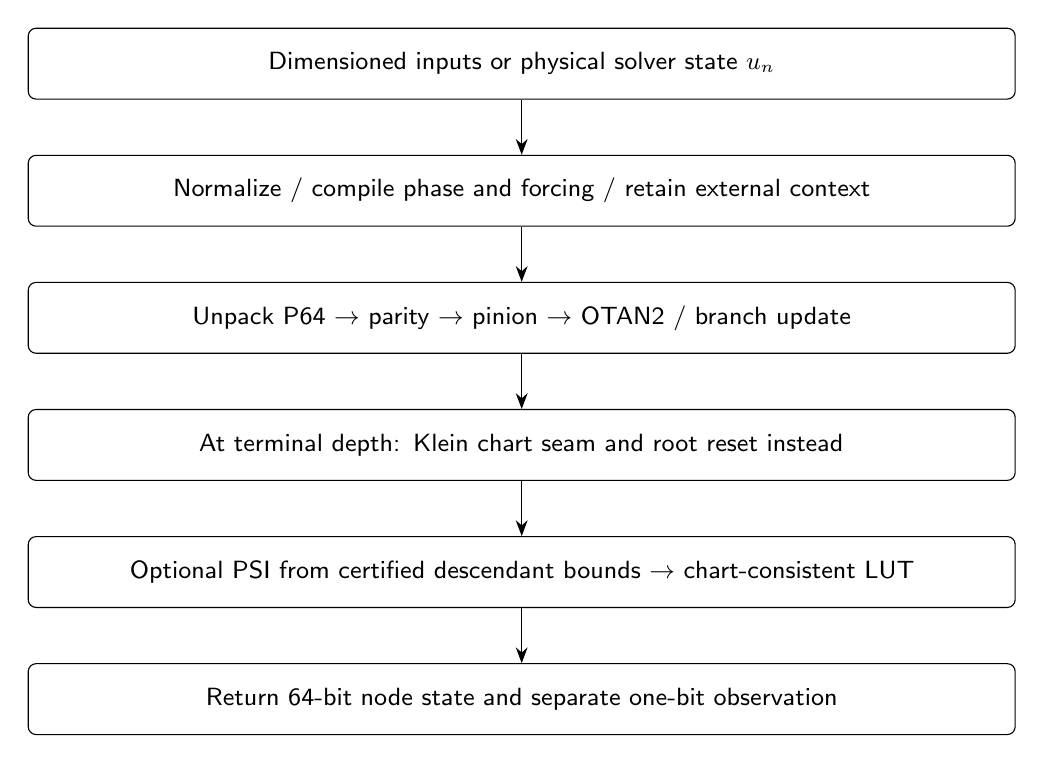
\begin{tikzpicture}[node distance=7mm,
 b/.style={draw,rounded corners=1mm,align=center,text width=12.3cm,minimum height=9mm,font=\small\sffamily},
 >={Stealth[length=2mm]}]
\node[b] (a) {Dimensioned inputs or physical solver state $u_n$};
\node[b,below=of a] (b) {Normalize / compile phase and forcing / retain external context};
\node[b,below=of b] (c) {Unpack P64 $\rightarrow$ parity $\rightarrow$ pinion $\rightarrow$ OTAN2 / branch update};
\node[b,below=of c] (d) {At terminal depth: Klein chart seam and root reset instead};
\node[b,below=of d] (e) {Optional PSI from certified descendant bounds $\rightarrow$ chart-consistent LUT};
\node[b,below=of e] (f) {Return 64-bit node state and separate one-bit observation};
\draw[->] (a)--(b);\draw[->] (b)--(c);\draw[->] (c)--(d);
\draw[->] (d)--(e);\draw[->] (e)--(f);
\end{tikzpicture}
\end{center}
The sequential drawing shows stage ownership; the terminal stage is an alternative to the nonterminal branch update. The output is a sampled bitstream. Omitting ray casting and triangle rasterization does not eliminate sampling or quantization.

\onepage
\section{Physical-equation supplement and coupling adapters}
\label{sec:physics}
\tagline{Classification: E for governing equations; D for their WANTWOMAN adapters. Units and initial/boundary conditions are part of each model.}

\subsection{SI constants and parameter ownership}
The SI fixes the numerical values of its defining constants. The following values used in this supplement are exact in SI \cite{bipm}:
\begin{align}
c&=299\,792\,458\ \mathrm{m\,s^{-1}},\\
h_{\rm P}&=6.62607015\times10^{-34}\ \mathrm{J\,s},\qquad \hbar=h_{\rm P}/(2\pi),\\
e&=1.602176634\times10^{-19}\ \mathrm C,\\
k_B&=1.380649\times10^{-23}\ \mathrm{J\,K^{-1}}.
\end{align}
Masses, spring and damping constants, diffusion coefficients, material properties, charge/current distributions, $G$, initial data and boundary data remain explicit model inputs. The symbols $\epsilon_0$ and $\mu_0$ are kept symbolic and obey $c^{-2}=\epsilon_0\mu_0$; no obsolete exact numerical value is assigned to either.

\subsection{Newtonian mechanics and the oscillator channel}
For constant mass, Newtonian motion is \cite[Ch.~9]{newton}
\begin{equation}
\dot{\bm x}=\bm p/m,\qquad \dot{\bm p}=\bm F,\qquad
\bm F=-\nabla V\quad\text{for a conservative potential}.
\label{eq:newton}
\end{equation}
Position is in metres, momentum in $\mathrm{kg\,m\,s^{-1}}$, force in newtons and $V$ in joules. Given $\bm x(0),\bm p(0)$ and a force law, a node nucleus can be attached to the resulting trajectory $\bm P_i(t)$.

The damped, driven oscillator is \cite[Sec.~23--2]{oscillation}
\begin{equation}
m\ddot x+b\dot x+kx=F_0\cos(\omega t+\beta),\qquad
\omega_0=\sqrt{k/m},\qquad
\zeta=\frac{b}{2\sqrt{mk}}.
\end{equation}
Its input units are $b$ in $\mathrm{kg\,s^{-1}}$, $k$ in $\mathrm{N\,m^{-1}}$, $\omega$ in radians per second and $F_0$ in newtons. WANTWOMAN uses a normalized displacement as a forcing channel,
\begin{equation}
\gamma_n=\clip_{[-31,31]}\bigl(\round(31x_n/L_*)\bigr).
\end{equation}
A measured frequency or a solved oscillator phase sets the phase adapter independently; choosing a nearby rational clock introduces a quantified period error.

For the undamped unit-normalized case, define $p=dx/d\tau$ and use the specified kick--drift step
\begin{equation}
p_{n+1}=p_n-hx_n,\qquad x_{n+1}=x_n+hp_{n+1}.
\label{eq:symplectic}
\end{equation}
Before rounding, its update matrix has determinant one and trace $2-h^2$; its eigenvalues lie on the unit circle for $0<h<2$. The modified quadratic
\begin{equation}
\widetilde H_h=\tfrac12(x^2+p^2-hxp)
\label{eq:modifiedenergy}
\end{equation}
is invariant under the exact arithmetic step, as direct substitution verifies. Fixed-point rounding introduces a separately measured invariant residual.

\subsection{Variational and Hamiltonian form}
A reusable mechanics/field interface uses an action \cite[Ch.~19]{action}
\begin{equation}
\mathcal S[q]=\int L(q,\dot q,t)\,dt,\qquad
\frac{d}{dt}\frac{\partial L}{\partial\dot q_i}-\frac{\partial L}{\partial q_i}=0.
\end{equation}
When the velocity-to-momentum map is invertible, define $p_i=\partial L/\partial\dot q_i$ and $\mathcal H=\sum_i p_i\dot q_i-L$; differentiation gives
\begin{equation}
\dot q_i=\frac{\partial\mathcal H}{\partial p_i},\qquad
\dot p_i=-\frac{\partial\mathcal H}{\partial q_i}.
\end{equation}
For fields, replace $L$ by a density $\mathcal L(u,\partial_\mu u,x)$:
\begin{equation}
\frac{\partial\mathcal L}{\partial u}
-\partial_\mu\!\left(\frac{\partial\mathcal L}{\partial(\partial_\mu u)}\right)=0.
\end{equation}
This gives a consistent external solver contract. The determinant property of the four-feature pinion operator is not a substitute for the symplectic conditions on a Hamiltonian integrator.

\subsection{Conservation, diffusion and heat transport}
A transported density $u$ and flux $\bm J_u$ satisfy local balance
\begin{equation}
\partial_tu+\nabla\cdot\bm J_u=s_u.
\label{eq:continuity}
\end{equation}
For a conserved density, $s_u=0$. The charge case follows from Maxwell's equations \cite{maxwell}; integrating over a cell gives its inventory change as minus net outward flux. With Fick's constitutive law $\bm J_u=-D\nabla u$, the constant-$D$ transport equation is
\begin{equation}
\partial_tu=D\nabla^2u+s_u,\qquad [D]=\mathrm{m^2\,s^{-1}}.
\end{equation}
Fourier heat flux is $\bm q_h=-k_{\rm th}\nabla T$, giving
\begin{equation}
\rho_m c_p\partial_tT=\nabla\cdot(k_{\rm th}\nabla T)+Q_h.
\end{equation}
Diffusive and conductive flux laws are described in the cited kinetic treatment \cite[Secs.~43--5 and 43--6]{diffusion}. Here $c_p$ is $\mathrm{J\,kg^{-1}\,K^{-1}}$, $k_{\rm th}$ is $\mathrm{W\,m^{-1}\,K^{-1}}$ and $Q_h$ is $\mathrm{W\,m^{-3}}$.

A concrete constant-$D$, one-dimensional stencil is
\begin{equation}
u_i^{n+1}=(1-2\lambda)u_i^n+\lambda u_{i-1}^n+\lambda u_{i+1}^n+h s_i^n,
\quad\lambda=Dh/(\Delta x)^2.
\end{equation}
For $0\le\lambda\le1/2$ and zero source, this is a convex combination, hence it preserves positivity and the range of the previous samples. With periodic boundaries, summing over $i$ also proves exact mass conservation before rounding. A $\lambda=1/4$ compile uses shifts. Thresholding $u$ before the flux calculation would discard the amplitude needed for this balance; P64 therefore observes the solver rather than replacing its field array with one bit.

\subsection{Waves and electromagnetism}
In a homogeneous vacuum, Maxwell's equations and the Lorentz force are \cite[Ch.~18]{maxwell}
\begin{align}
\nabla\cdot\bm E&=\rho_e/\epsilon_0,&\quad\nabla\cdot\bm B&=0,\\
\nabla\times\bm E&=-\partial_t\bm B,&
\nabla\times\bm B&=\mu_0\bm J+\mu_0\epsilon_0\partial_t\bm E,\\
\bm F&=q(\bm E+\bm v\times\bm B).&&
\end{align}
In a source-free region they imply
\begin{equation}
\partial_t^2\bm E=c^2\nabla^2\bm E,\qquad
\partial_t^2\bm B=c^2\nabla^2\bm B.
\end{equation}
$\bm E$ has units $\mathrm{V\,m^{-1}}$, $\bm B$ tesla, $\rho_e$ $\mathrm{C\,m^{-3}}$, and $\bm J$ $\mathrm{A\,m^{-2}}$. The equations require compatible initial fields and boundary/source data. In particular, the divergence constraints must be maintained by the selected solver.

A general scalar wave adapter uses
\begin{equation}
\partial_t^2u-c_w^2\nabla^2u=s,
\qquad
u_i^{n+1}=2u_i^n-u_i^{n-1}+\lambda_w^2(u_{i+1}^n-2u_i^n+u_{i-1}^n)+h^2s_i^n,
\end{equation}
where $\lambda_w=c_wh/\Delta x$. Substitution of a Fourier mode shows the homogeneous one-dimensional scheme has no exponentially growing mode when $|\lambda_w|\le1$; strict inequality avoids the defective highest-frequency endpoint. Its array samples can drive a phase or a threshold input. An orientation reversal in P64 is a chart operation, not the electric/magnetic duality transformation.

\subsection{Quantum amplitude evolution and observation}
For a single nonrelativistic spinless particle with real potential $V$, the Schr\"odinger equation is \cite[Sec.~16--5]{quantum}
\begin{equation}
i\hbar\partial_t\psi=
\left[-\frac{\hbar^2}{2m}\nabla^2+V\right]\psi,
\qquad\int |\psi|^2\,d^3x=1.
\end{equation}
In three dimensions the normalized amplitude has units $\mathrm{m^{-3/2}}$. A spatial discretization with Hermitian Hamiltonian matrix $H$ admits the Cayley step
\begin{equation}
\left(I+\frac{ihH}{2\hbar}\right)\psi_{n+1}
=\left(I-\frac{ihH}{2\hbar}\right)\psi_n.
\end{equation}
Diagonalizing the Hermitian matrix shows each eigenmode is multiplied by $(1-ia)/(1+ia)$ for real $a$, of unit magnitude. Hence this step preserves the discrete norm before solver/rounding error.

A WANTWOMAN observation may threshold a cell probability
$P_i=\int_{C_i}|\psi|^2\,d^3x$ or encode it as a pulse density. That decision does not preserve the complex phase of $\psi$. The complex solver state remains in $\mathcal C_n$, while $O_n$ is the selected classical record. This supplement specifies the adapter; the supplied Python demo does not implement a quantum solver.

\subsection{Relativistic dynamics and geometric gravity}
For special-relativistic motion in flat spacetime \cite[Ch.~15]{relativity},
\begin{equation}
\gamma_v=(1-v^2/c^2)^{-1/2},\quad
\bm p=\gamma_v m\bm v,\quad E=\gamma_v mc^2,\quad
E^2=c^2\bm p\cdot\bm p+m^2c^4.
\end{equation}
The source's four-feature pinion coordinate must not be substituted for $(ct,\bm x)$ without a separately defined spacetime adapter.

For general relativity, use metric signature $(-,+,+,+)$, $x^0=ct$, the Levi-Civita connection and the standard Einstein tensor convention \cite[Secs.~3--4]{carroll}:
\begin{align}
R_{\mu\nu}-\tfrac12Rg_{\mu\nu}+\Lambda g_{\mu\nu}
&=\frac{8\pi G}{c^4}T_{\mu\nu},\\
\frac{d^2x^\mu}{d\lambda^2}+\Gamma^\mu_{\alpha\beta}
\frac{dx^\alpha}{d\lambda}\frac{dx^\beta}{d\lambda}&=0.
\end{align}
The second equation describes a freely falling trajectory with affine parameter $\lambda$. The scalar curvature $R$ and $\Lambda$ have units $\mathrm{m^{-2}}$ when the coordinates have length units. Metric components, stress-energy, constraint-satisfying initial data, coordinate gauge and boundary conditions belong to the selected gravity problem. A compact node record can index their normalized samples; the metric is not supplied by the mere presence of a Klein seam.

\subsection{Crop-water and event-progress adapters}
The source's crop channel can be connected to physical environmental inputs instead of a free-running nominal period. FAO's AquaCrop calculation scheme links canopy cover, crop transpiration, biomass and harvest index. In well-watered conditions its stated transpiration relation is \cite{fao}
\begin{equation}
\mathrm{Tr}=K_{c\mathrm{Tr}}\,\mathrm{ET}_0,
\end{equation}
with dimensionless coefficient $K_{c\mathrm{Tr}}$ and both water-flux quantities in the same depth-per-time unit. A simple explicitly chosen root-zone water-balance adapter is
\begin{equation}
\dot S_w=P+I-\mathrm{ET}-R_{\rm off}-D_{\rm drain}.
\end{equation}
All right-hand terms must use the same units, such as $\mathrm{mm\,day^{-1}}$, and the soil-water store $S_w$ is in millimetres. This balance is a separate completion, not a claim to implement the full AquaCrop model. A measured or fitted progress variable can then supply $\psi_c$ and a soil-water threshold can supply a one-bit observation.

For the source's chromosome labels, choose two symbolic tokens $L_0,L_1$ and let $b(L_0)=0$, $b(L_1)=1$; the exact swap is $b_\chi(L)=b(L)\oplus\chi$. Using the strings ``XX'' and ``XY'' as those tokens changes a label lookup, not chromosomes, sex or reproductive physiology. Event/cycle records supply timing data; no clinical prediction follows from the toggle alone.

\section{Approximation, quantization and measurement criteria}
\label{sec:error}
\tagline{Classification: D + P. Error bounds specify their encoder, solver, norm and hypotheses.}

\subsection{Quantizer errors with explicit conditions}
For an unclipped scalar nearest-neighbor quantizer with step $\Delta u$,
\begin{equation}
|\widehat u-u|\le\Delta u/2.
\end{equation}
For the unclipped radial rule \eqref{eq:radial},
\begin{equation}
|\widehat\ell-\ell|\le\Delta\ell/2,\qquad
\left|\frac{\widehat r_{\rm phys}}{r_{\rm phys}}-1\right|
\le2^{\Delta\ell/2}-1.
\end{equation}
Nearest rounding to 2048 angular bins has circular error at most $\pi/2048$. A 128-bin nearest-center boundary compiler has angular mismatch at most $\pi/128$; the floor-address rule assigns a bin, so this bound uses the bin's center, not its lower edge. Clipping or periodic wrap at a nonperiodic physical boundary adds a different error and must be reported independently.

If a physical scalar observable $f$ has Lipschitz constant $L_f$ in the chosen metric, coordinate error $\epsilon_x$ and field/threshold errors $\epsilon_f,\epsilon_\tau$ imply
\begin{equation}
\epsilon_{\rm total}\le L_f\epsilon_x+\epsilon_f+\epsilon_\tau.
\end{equation}
Its binary threshold decision is stable wherever
$|f(\bm x)-\tau|>\epsilon_{\rm total}$. Near the threshold, a small numerical error can change the bit even when the underlying scalar approximation is accurate.

\subsection{A general finite-horizon error estimate}
Suppose an exact step $F_h$ is Lipschitz with constant $1+hL$, and the selected numerical/encoding step has total one-step error at most $\delta$. Then
\begin{equation}
e_{n+1}\le(1+hL)e_n+\delta,
\end{equation}
so induction gives, for $L>0$,
\begin{equation}
e_N\le(1+hL)^N e_0+
\delta\frac{(1+hL)^N-1}{hL}.
\end{equation}
For $L=0$, the corresponding bound is $e_N\le e_0+N\delta$. This theorem requires the stated smoothness/Lipschitz contract. A wrapped or thresholded code sequence is not automatically Lipschitz across its jumps.

\subsection{One-bit pulse density preserves an average, not each amplitude}
For normalized samples $a_n\in[0,1]$, set
\begin{equation}
s_n=e_n+a_n,\qquad b_n=\ind\{s_n\ge1\},\qquad
 e_{n+1}=s_n-b_n,\quad e_0=0.
\label{eq:sd}
\end{equation}
Then $0\le e_n<1$ and telescoping gives
\begin{equation}
\left|\frac1N\sum_{n=0}^{N-1}b_n-\frac1N\sum_{n=0}^{N-1}a_n\right|
=\frac{|e_N-e_0|}{N}<\frac1N.
\end{equation}
The implementation uses $a_n=A_n/Q$ and an integer residual, so the identity is exact for the supplied integers. For a signed observable $x/L_*\in[-1,1]$, choose $a=(x/L_*+1)/2$. Its reconstructed block mean has corresponding encoding error below $2L_*/N$, before input quantization or clipping. The oscillator pulse-density stream is distinct from the polar-membership stream.

\subsection{Physical validation record}
Each application should record the physical equation and its regime, measured inputs and units, initial/boundary conditions, normalization scales, complete word profile, LUT provenance, and solver/quantizer settings. Compare predicted unthresholded observables against measurements before comparing binary outputs. Report numerical residuals, conservation drift, saturation counts and parameter-fit error separately. No such experimental measurement set is present in the uploaded source; the numerical results below are a synthetic reproducibility benchmark.

\section{Executed benchmark and conformance results}
\label{sec:results}
\tagline{Classification: T. These values are computed by code/reproduce.py and saved in results/numerical\_report.json.}

\subsection{Physical benchmark configuration}
The solved benchmark is the unforced oscillator with $m=1\ \mathrm{kg}$, $k=1\ \mathrm{N\,m^{-1}}$, $x(0)=1\ \mathrm m$, $p(0)=0$, $T_*=1\ \mathrm s$ and $L_*=1\ \mathrm m$. Its exact comparison solution is
\begin{equation}
x(t)=\cos t\ \mathrm m,\qquad p(t)=-\sin t\ \mathrm{kg\,m\,s^{-1}}.
\end{equation}
The reference solver applies \eqref{eq:symplectic} with $h=1/128\ \mathrm s$ and Q24 normalized state, over 4096 updates (32 seconds). Reference trigonometry is used only for benchmark comparison, outside the integer kernel.

\begin{tabularx}{\textwidth}{@{}Y p{56mm}@{}}
\toprule
Executed quantity & Result\\
\midrule
Maximum absolute position error & $0.00398409718\ \mathrm m$\\
Maximum absolute momentum error & $0.0000826205370\ \mathrm{kg\,m\,s^{-1}}$\\
Maximum ordinary-energy error & $0.00196116128\ \mathrm J$\\
Maximum modified-energy residual, \eqref{eq:modifiedenergy} & $6.87441319\times10^{-7}\ \mathrm J$\\
Pulse-density mean error for quantized/clipped input & $7.22866534\times10^{-5}$\\
Proved bound for 4096-sample normalized mean & $1/4096=0.000244140625$\\
Node-membership ones in 4096 output bits & 2398\\
Bytes per binary output file & 512\\
\bottomrule
\end{tabularx}
The P64 demonstration uses channel 3 (composite/user), $\chi=0$, alternating branch input $b_n=n\bmod2$, the triangular table \eqref{eq:demolut}, strict0 OTAN2 and the oscillator-derived integer forcing. Its independent rational phase clock uses 804 ticks: $804/128=6.28125\ \mathrm s$, compared with the oscillator period $2\pi\ \mathrm s$. The relative period difference is $3.08013704\times10^{-4}$.

The first and last returned words are respectively
\begin{center}\ttfamily
2A22D3EF039080B3\qquad 43599C16FAC00A73.
\end{center}
These values, all decoded fields, oscillator samples and both output bits appear in \texttt{data/trace.csv}. The file records 4096 pre-step physical samples over $0\le t<32$ seconds; the solver report also includes the terminal physical state at 32 seconds.

\subsection{Time-step refinement}
With Q24 held fixed and an eight-second comparison window:
\begin{center}
\begin{tabular}{@{}rr@{}}
\toprule
Time step (seconds) & Maximum position error (metres)\\
\midrule
$1/64$ & 0.00789295267\\
$1/128$ & 0.00392665229\\
$1/256$ & 0.00195868864\\
\bottomrule
\end{tabular}
\end{center}
The errors approximately halve when the step halves, as expected for this first-order method. These are numerical measurements of a specified synthetic case, not experimental calibration of the framework.

\subsection{Checks actually run}
The package contains \textbf{28 passing unittest cases}. They include complete 10/11-bit sign decoding; 1500 word round trips; mask isolation; local negation; the source's ineffective mask and carry-producing toggle; exact Hadamard identities; fixed-pinion rounding against an independent rational reference; all 4096 $(r,O)$ strict0 inputs; both mixer permutations; all 4096 $(\vartheta,\kappa)$ seam states; terminal reset; 4096 deterministic kernel updates; a rational clock cycle; rational affine bounds; safe pruning against an enumerated tree; bit packing/padding; exact pulse-density conservation; and time-step refinement.

Those tests establish the listed conformance properties. They do not execute Maxwell, quantum, relativity, crop-water or general-purpose scene solvers; those parts of Section~\ref{sec:physics} are equation/adapter specifications. The package's implemented physical solver is the oscillator demonstration.

\onepage
\section{Source-to-formalization reconciliation ledger}
\label{sec:ledger}
\tagline{The source is preserved, not silently rewritten. Locations refer to the uploaded 21-page PDF.}

\small
\begin{longtable}{@{}>{\raggedright\arraybackslash}p{16mm}>{\raggedright\arraybackslash}p{51mm}>{\raggedright\arraybackslash}p{90mm}@{}}
\toprule
Source & Source statement or ambiguity & Normative treatment in WANTWOMAN\\
\midrule
\endfirsthead
\toprule
Source & Source statement or ambiguity & Normative treatment in WANTWOMAN\\
\midrule
\endhead
p.~1 & 3.6, 36, $\phi$, $2\pi$, Fibonacci and birth date are associated without a single equation. & Supply typed angular identities, Fibonacci recursion, unit conversion and a civil-date anchor; their different roles remain explicit.\\
p.~2, 4 & A Fourier transform is described as a 0--1 sweep. & Define phase and Fourier transform separately; retain FT as the field's historical name.\\
p.~4 & $\log|\sin\cdot\cos\cdot\sin|$ can diverge at zero. & Add a named positive floor $\epsilon$ and specify jitter/gain.\\
p.~7 & Culling argument assumes $\Gamma\ge0$. & Do not use that sign assumption; the regularized logarithm can be negative.\\
p.~2--5 & ``1-bit SDF'' is used for Boolean inequalities and lookup tests. & Treat it as occupancy; require a separate metric for true signed distances.\\
p.~2, 5 & Apex test omits $z$; pyramid is unbounded; sphere LUT is incomplete. & State completed finite predicates and the data required for 2D versus 3D boundaries.\\
p.~3, 5 & Scene composition alternates between XOR and OR. & Preserve both as different policies: parity/symmetric difference versus union.\\
p.~5, 9 & Normalized matrix coefficients become $\pm1$ in code. & Use $H_4=M/2$; identify the unnormalized $M$ separately.\\
p.~5 & Hadamard orthogonality is used to claim preservation by the full pinion map. & Prove orthogonality only for $H_4$ and four-volume magnitude preservation for $A=D_\phi H_4$; give its non-unit singular values.\\
p.~5, 9 & Shifts and cross-additions are called exact golden-ratio operations. & Specify Q16 coefficients, ordered rounding and their numerical errors.\\
p.~6--7, 10 & Parent bounds, depth and a claimed positive-definiteness argument are used for pruning. & Require whole-descendant enclosures; prove the slit test by containment.\\
p.~6 & Eigenvalue $-1$ and a two-axis sign flip are called a Klein bottle. & Supply an actual quotient relation and chart seam; keep the source's transformations distinct.\\
p.~7--8 & Word schematic and detailed table disagree. & Use the complete p.~8 table as allocation authority.\\
p.~8 & One-bit value is ANDed directly with a high-bit mask. & Show the result is zero; use field-local replacement or a properly expanded mask.\\
p.~9, 12 & Complement masks are called two's-complement negation. & Define complement, modular negation and signed-range handling separately.\\
p.~12 & Adding 4 is described as toggling $\kappa$. & XOR bit 2, avoiding carries into the LUT.\\
p.~11--12 & Lowest-bit parity is described as spatial parity; left-to-right comments accompany native C syntax. & Identify the actual three metadata bits and compile the left fold using explicit statements/parentheses.\\
p.~11 & One-bit shifts stand in for golden leaf progression. & Treat shifts as doubling/halving only; specify golden phase quantization independently.\\
p.~13, 20 & X/Y slots are reinterpreted as log radius/angle; final diagram omits Z. & Introduce the external P64 profile and retain Z as an axial auxiliary.\\
p.~14 & Radial inversion plus half-turn is assigned Klein topology. & Preserve it as a separate radial involution; use the quotient seam for Klein chart closure.\\
p.~15 & A 7-bit LUT address is described as a 1-bit LUT. & Store 128 radial thresholds with 11-bit values; only the comparison result is one bit.\\
p.~16 & Bit 0 is read as occupancy although already allocated to the cycle selector. & Return and feed back $O$ separately from $W$.\\
p.~16 & Literal 0-order OTAN2 and C-precedence OTAN2 differ. & Implement strict0's two-phase rule and the full-code mixer as separately named modes.\\
p.~16--17 & Finite words/bit shifts are said to create infinite geometric volume or exact infinite nesting. & Specify abstract unbounded tree addresses separately from bounded-depth records and finite-state recurrence.\\
p.~2, 4, 8 & An XX/XY label inversion is given biological meaning. & Formalize the token swap as XOR; physiological timing requires its own measurements/model.\\
\bottomrule
\end{longtable}
\normalsize

\section{Archive contents and reproduction}
\label{sec:reproduce}
\tagline{All paths below are relative to the top-level WANTWOMAN directory inside WANTWOMAN.zip.}

\begin{tabularx}{\textwidth}{@{}p{64mm}Y@{}}
\toprule
Path & Contents\\
\midrule
\texttt{WANTWOMAN.pdf} & This formalization.\\
\texttt{source/WANTWOMAN.tex} & Editable LaTeX source with equations, proofs and bibliography.\\
\texttt{code/wantwoman.py} & P64 kernel, clocks, OTAN2 variants, seam maps, interval bounds, bitstream utilities and integer oscillator.\\
\texttt{code/reproduce.py} & Synthetic trace, binary streams and numerical report generation.\\
\texttt{tests/test\_wantwoman.py} & The 28 conformance/numerical test cases.\\
\texttt{data/} & Trace CSV, explicit LUT, field masks, two binary streams and stream metadata.\\
\texttt{results/} & Executed test log and numerical report.\\
\texttt{original/source.pdf} & Unmodified copy of the supplied 21-page source.\\
\texttt{REFERENCES.json} & Source titles, publishers, URLs and uses.\\
\texttt{README.md} & Commands, profile contract and output interpretation.\\
\texttt{MANIFEST.sha256} & Integrity hashes for packaged files, excluding the manifest itself.\\
\bottomrule
\end{tabularx}

The Python implementation uses only the standard library and was executed with Python 3.13.5. Its syntax supports Python 3.10 or later. From the archive root:
\begin{lstlisting}[language=bash]
python -m unittest discover -s tests -v
python code/reproduce.py
\end{lstlisting}
To rebuild the document using a TeX distribution with the listed packages:
\begin{lstlisting}[language=bash]
cd source
pdflatex -interaction=nonstopmode -halt-on-error WANTWOMAN.tex
pdflatex -interaction=nonstopmode -halt-on-error WANTWOMAN.tex
\end{lstlisting}
No font binaries are bundled. TeX uses its installed Latin Modern fonts. The document contains ordinary text and vector mathematics rather than scanned equations.

\subsection{Serialization contract}
\texttt{polar\_occupancy.bin} and \texttt{oscillator\_sigma\_delta.bin} are raw bits, packed most-significant-bit first in each byte. Any incomplete final byte is padded with zeroes on the right. The valid-bit count is recorded separately; both bundled streams contain exactly 4096 valid bits. Word hexadecimal values in the trace are unsigned 16-character representations of P64 records, not a native-memory byte dump. A future binary-word transport must declare byte order.

\subsection{A reproducible author configuration}
The document attribution carries the supplied identity string and date. The node demonstration itself begins with
\begin{equation}
(\chi,r,\vartheta,z,\Phi,d,p,j_L,\kappa,\Xi)
=(0,1024,0,0,0,0,0,0,0,3),\qquad O_0=0.
\end{equation}
Personal metadata is not injected into force laws, material constants or biological phase estimates. This configuration, the arithmetic definitions, the explicit LUT and the external clock fully determine the supplied demonstration trace.

\onepage
\section*{References}
\addcontentsline{toc}{section}{References}
\tagline{External references were accessed on 15 September 2026. Click a title to open its publisher or author-hosted source.}
\begingroup
\renewcommand{\section}[2]{}
\begin{thebibliography}{99}
\bibitem[S0]{source}
Tom Klootwijk, supplied source artifact. \emph{3.6-phi-2pi-fibonacci-36-10---07---1990-gregorian-calander-Tom-Klootwijk.pdf}. 21 pages, user-uploaded exported dialogue. Preserved as \texttt{original/source.pdf}; provenance is the conversation upload, not an externally verified publication.

\bibitem[M1]{hatcher}
Allen Hatcher. \href{https://pi.math.cornell.edu/~hatcher/Top/TopNotes.pdf}{\emph{Notes on Introductory Point-Set Topology}}. Cornell University, Chapter 4, pp.~44--45. Supports the rectangle/quotient construction of the Klein bottle.

\bibitem[U1]{bipm}
Bureau International des Poids et Mesures. \href{https://www.bipm.org/en/measurement-units/si-defining-constants}{\emph{The International System of Units: Defining constants}}. Supports the exact SI values used in Section~\ref{sec:physics}.

\bibitem[P1]{newton}
Richard P. Feynman, Robert B. Leighton and Matthew Sands. \href{https://www.feynmanlectures.caltech.edu/I_09.html}{\emph{The Feynman Lectures on Physics}, Vol.~I, Ch.~9: Newton's Laws of Dynamics}. Caltech online edition.

\bibitem[P2]{oscillation}
Feynman, Leighton and Sands. \href{https://www.feynmanlectures.caltech.edu/I_23.html}{\emph{The Feynman Lectures on Physics}, Vol.~I, Ch.~23: Resonance}. In particular Sec.~23--2 on a forced oscillator with damping. Caltech online edition.

\bibitem[P3]{action}
Feynman, Leighton and Sands. \href{https://www.feynmanlectures.caltech.edu/II_19.html}{\emph{The Feynman Lectures on Physics}, Vol.~II, Ch.~19: The Principle of Least Action}. Caltech online edition.

\bibitem[P4]{diffusion}
Feynman, Leighton and Sands. \href{https://www.feynmanlectures.caltech.edu/I_43.html}{\emph{The Feynman Lectures on Physics}, Vol.~I, Ch.~43: Diffusion}. In particular Secs.~43--5 and 43--6. Caltech online edition.

\bibitem[P5]{maxwell}
Feynman, Leighton and Sands. \href{https://www.feynmanlectures.caltech.edu/II_18.html}{\emph{The Feynman Lectures on Physics}, Vol.~II, Ch.~18: The Maxwell Equations}. Caltech online edition.

\bibitem[P6]{quantum}
Feynman, Leighton and Sands. \href{https://www.feynmanlectures.caltech.edu/III_16.html}{\emph{The Feynman Lectures on Physics}, Vol.~III, Ch.~16: The Dependence of Amplitudes on Position}. In particular Sec.~16--5, the Schr\"odinger equation. Caltech online edition.

\bibitem[P7]{relativity}
Feynman, Leighton and Sands. \href{https://www.feynmanlectures.caltech.edu/I_15.html}{\emph{The Feynman Lectures on Physics}, Vol.~I, Ch.~15: The Special Theory of Relativity}. Caltech online edition.

\bibitem[P8]{carroll}
Sean M. Carroll. \href{https://arxiv.org/abs/gr-qc/9712019}{\emph{Lecture Notes on General Relativity}}. arXiv:gr-qc/9712019 (1997), especially Secs.~3--4. DOI: 10.48550/arXiv.gr-qc/9712019. The supplement restores SI factors of $c$ in equations commonly written in units $c=1$.

\bibitem[A1]{fao}
Food and Agriculture Organization of the United Nations. \href{https://www.fao.org/aquacrop/overview/calculation-scheme/en/}{\emph{AquaCrop: Calculation scheme}}. Supports the canopy/transpiration/biomass framework and the well-watered transpiration relation; the simple water-balance adapter in this edition is identified separately.
\end{thebibliography}
\endgroup
\end{document}
